\documentclass[tikz,border=8pt]{standalone}
\usepackage[utf8]{inputenc}
\usepackage[T1]{fontenc}
\usepackage{amsmath,amssymb}
\usetikzlibrary{arrows.meta,positioning,calc,shapes.geometric}

\definecolor{bgdark}{HTML}{0F172A}
\definecolor{paneldark}{HTML}{1E293B}
\definecolor{gridline}{HTML}{334155}
\definecolor{cellbg}{HTML}{0B1120}
\definecolor{agentblue}{HTML}{38BDF8}
\definecolor{obsred}{HTML}{EF4444}
\definecolor{goalgreen}{HTML}{22C55E}
\definecolor{threatamber}{HTML}{F59E0B}
\definecolor{textlight}{HTML}{F8FAFC}
\definecolor{textmuted}{HTML}{94A3B8}

\newcommand{\drawboardbase}[1]{
    \fill[paneldark, rounded corners=6pt] (-0.65, -2.15) rectangle (8.65, 8.95);
    \draw[gridline, line width=0.8pt, rounded corners=6pt] (-0.65, -2.15) rectangle (8.65, 8.95);
    \node[anchor=west, text=textlight, font=\sffamily\bfseries\scriptsize] at (-0.42, 8.58) {#1};
    \fill[cellbg] (0, 0) rectangle (8, 8);
    \fill[agentblue, fill opacity=0.16] (0, 7) rectangle (1, 8);
    \node[anchor=north, inner sep=0.8pt, scale=0.78, text=textmuted, font=\sffamily\bfseries\tiny] at (0.5, 7.97) {START};
    \fill[goalgreen, fill opacity=0.26] (7, 0) rectangle (8, 1);
    \node[anchor=south, inner sep=0.8pt, scale=0.78, text=goalgreen, font=\sffamily\bfseries\tiny] at (7.5, 0.03) {GOAL};
    \draw[gridline, line width=0.45pt] (0, 0) grid (8, 8);
    \draw[gridline, line width=0.9pt] (0, 0) rectangle (8, 8);
    \foreach \i in {0,...,7} {
        \node[text=textmuted, font=\sffamily\tiny] at (\i+0.5, 8.18) {\i};
        \node[text=textmuted, font=\sffamily\tiny] at (-0.22, 7.5-\i) {\i};
    }
}

\newcommand{\drawobs}[2]{
    \pgfmathsetmacro{\ox}{#2}
    \pgfmathsetmacro{\oy}{7-#1}
    \fill[obsred, rounded corners=2.2pt] (\ox+0.18, \oy+0.18) rectangle (\ox+0.82, \oy+0.82);
}

\newcommand{\drawagent}[3]{
    \pgfmathsetmacro{\ax}{#2+0.5}
    \pgfmathsetmacro{\ay}{7-#1+0.5}
    \pgfmathsetmacro{\rotangle}{-#3*90}
    \begin{scope}[shift={(\ax,\ay)}, rotate=\rotangle]
        \fill[agentblue] (0, 0.25) -- (0.21, -0.21) -- (0, -0.10) -- (-0.21, -0.21) -- cycle;
        \draw[white, line width=0.35pt] (0, 0.25) -- (0.21, -0.21) -- (0, -0.10) -- (-0.21, -0.21) -- cycle;
    \end{scope}
}

\newcommand{\drawhud}[5]{
    \fill[bgdark, rounded corners=3pt] (-0.45, -1.95) rectangle (8.45, -0.22);
    \draw[gridline, line width=0.5pt, rounded corners=3pt] (-0.45, -1.95) rectangle (8.45, -0.22);
    \node[anchor=west, text=textmuted, font=\sffamily\tiny] at (-0.28, -0.52) {Paso/Ev.: \texttt{\textcolor{textlight}{#1}}};
    \node[anchor=west, text=textmuted, font=\sffamily\tiny] at (3.45, -0.52) {Acci\'on: \texttt{\textcolor{agentblue}{#2}}};
    \node[anchor=west, text=textmuted, font=\sffamily\tiny] at (-0.28, -1.05) {Recompensa Acum.: \texttt{\textcolor{#5}{#3}}};
    \node[anchor=west, text=textmuted, font=\sffamily\tiny] at (-0.28, -1.58) {Estado $s_Q=(x_a, y_a, \theta_a)$: \texttt{\textcolor{textlight}{#4}}};
}

\begin{document}
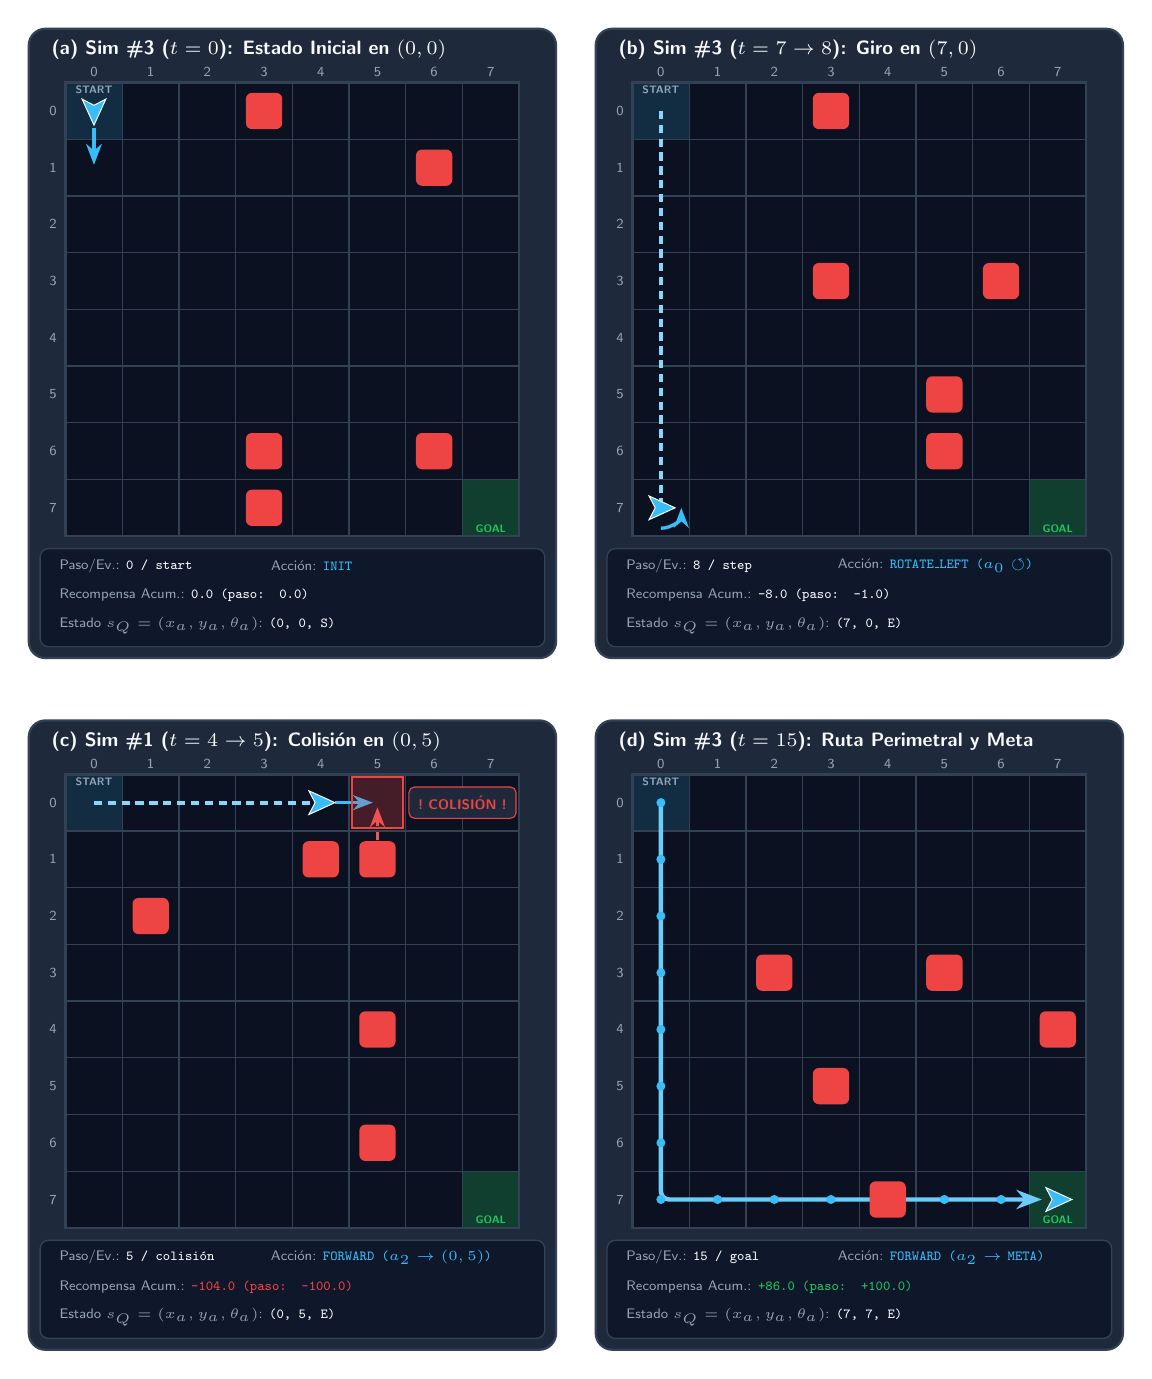
\begin{tikzpicture}[scale=0.72]

% =========================================================================
% PANEL (a): Sim #3 - Step 0 (Start at (0,0) facing SOUTH)
% =========================================================================
\begin{scope}[shift={(0, 0)}]
    \drawboardbase{(a) Sim \#3 ($t=0$): Estado Inicial en $(0,0)$}
    \drawobs{1}{6}
    \drawobs{6}{6}
    \drawobs{0}{3}
    \drawobs{7}{3}
    \drawobs{6}{3}
    \draw[-{Stealth[scale=0.9]}, agentblue, very thick] (0.5, 7.20) -- (0.5, 6.55);
    \drawagent{0}{0}{2}
    \drawhud{0 / start}{INIT}{0.0 (paso: 0.0)}{(0, 0, S)}{textlight}
\end{scope}

% =========================================================================
% PANEL (b): Sim #3 - Step 7 -> 8 (Corner turn at (7,0) SOUTH -> EAST)
% =========================================================================
\begin{scope}[shift={(10.0, 0)}]
    \drawboardbase{(b) Sim \#3 ($t=7 \to 8$): Giro en $(7,0)$}
    \draw[agentblue!60, line width=1.4pt, densely dashed] (0.5, 7.5) -- (0.5, 0.5);
    \drawobs{3}{6}
    \drawobs{5}{5}
    \drawobs{0}{3}
    \drawobs{3}{3}
    \drawobs{6}{5}
    \drawagent{7}{0}{1}
    \draw[-{Stealth[scale=0.85]}, agentblue, very thick] (0.5, 0.14) arc (-90:0:0.36);
    \drawhud{8 / step}{ROTATE\_LEFT ($a_0 \circlearrowleft$)}{-8.0 (paso: -1.0)}{(7, 0, E)}{textlight}
\end{scope}

% =========================================================================
% PANEL (c): Sim #1 - Step 4 -> 5 (Simultaneous collision at (0,5))
% =========================================================================
\begin{scope}[shift={(0, -12.2)}]
    \drawboardbase{(c) Sim \#1 ($t=4 \to 5$): Colisi\'on en $(0,5)$}
    \draw[agentblue!60, line width=1.4pt, densely dashed] (0.5, 7.5) -- (4.5, 7.5);
    \drawobs{2}{1}
    \drawobs{6}{5}
    \drawobs{1}{4}
    \drawobs{4}{5}
    \drawobs{1}{5}
    \draw[-{Stealth[scale=0.85]}, agentblue, very thick] (4.76, 7.5) -- (5.42, 7.5);
    \draw[-{Stealth[scale=0.85]}, obsred!90, very thick, densely dashed] (5.5, 6.84) -- (5.5, 7.42);
    \fill[obsred, fill opacity=0.25] (5.05, 7.05) rectangle (5.95, 7.95);
    \draw[obsred, thick] (5.05, 7.05) rectangle (5.95, 7.95);
    \node[draw=obsred, fill=paneldark, text=obsred, font=\sffamily\bfseries\tiny, rounded corners=2pt] at (7.0, 7.5) {!~COLISI\'ON~!};
    \drawagent{0}{4}{1}
    \drawhud{5 / colisi\'on}{FORWARD ($a_2 \to (0,5)$)}{-104.0 (paso: -100.0)}{(0, 5, E)}{obsred}
\end{scope}

% =========================================================================
% PANEL (d): Sim #3 - Step 15 (Optimal 15-step perimeter trajectory & Goal)
% =========================================================================
\begin{scope}[shift={(10.0, -12.2)}]
    \drawboardbase{(d) Sim \#3 ($t=15$): Ruta Perimetral y Meta}
    \draw[agentblue!75, line width=1.6pt, rounded corners=3pt, -{Stealth[scale=0.9]}]
        (0.5, 7.5) -- (0.5, 0.5) -- (7.22, 0.5);
    \foreach \px/\py in {0.5/7.5, 0.5/6.5, 0.5/5.5, 0.5/4.5, 0.5/3.5, 0.5/2.5, 0.5/1.5, 0.5/0.5, 1.5/0.5, 2.5/0.5, 3.5/0.5, 4.5/0.5, 5.5/0.5, 6.5/0.5} {
        \fill[agentblue] (\px, \py) circle (0.08);
    }
    \drawobs{4}{7}
    \drawobs{3}{5}
    \drawobs{3}{2}
    \drawobs{5}{3}
    \drawobs{7}{4}
    \drawagent{7}{7}{1}
    \drawhud{15 / goal}{FORWARD ($a_2 \to \text{META}$)}{+86.0 (paso: +100.0)}{(7, 7, E)}{goalgreen}
\end{scope}

\end{tikzpicture}
\end{document}
